%
% teil1.tex -- Beispiel-File für das Paper
%
% (c) 2020 Prof Dr Andreas Müller, Hochschule Rapperswil
%
% !TEX root = ../../buch.tex
% !TEX encoding = UTF-8
%
\section{Strömungsgleichungen\label{ueberschall:stroemungsgleichung}}
\kopfrechts{Strömungsgleichungen}
Wir untersuchen hier an einem einfachen Beispiel, 
illustriert in Abbildung~\ref{fig:wellblech},
die Strömung der Luft über ein gewelltes Blech,
welche eine kleine Störung hereinbringt.
% \documentclass{article}
% \usepackage{tikz}
% \usepackage{amsmath}

% \begin{document}
\begin{figure}
    \centering
    \resizebox{\textwidth}{!}{
    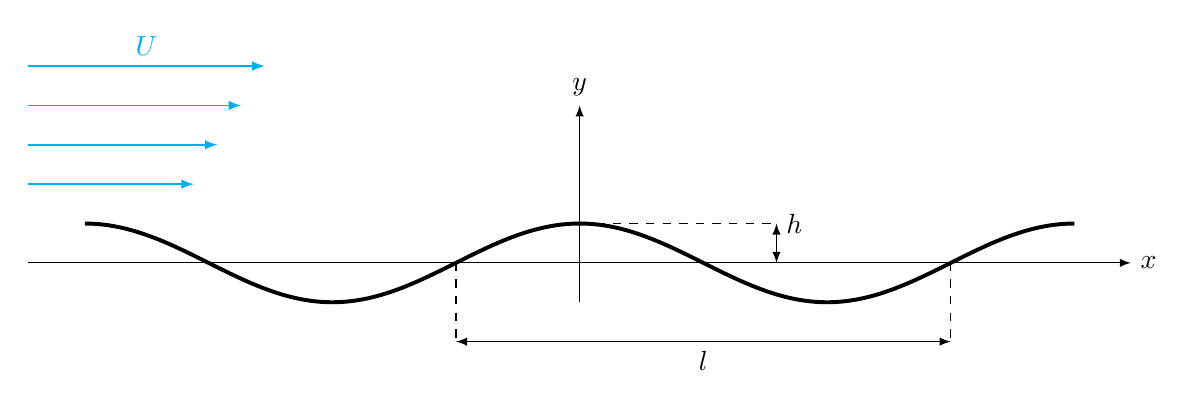
\begin{tikzpicture}[scale=1.0]
            % Achsen
        \def\startx{-7}
        \def\endx{-4}
        \def\starty{2.5}
        \def\ydis{0.5}
        \def\xenddis{0.3}
        \draw[->,>=latex] (-7, 0) -- (7, 0) node[right] {$x$};
        \draw[->,>=latex] (0, -0.5) -- (0, 2) node[above] {$y$};
        \draw[->,>=latex,cyan, line width=0.02cm] (\startx, \starty) -- (\endx, \starty) node[midway, yshift=0.25cm] {$U$};
        \draw[->,>=latex,cyan, line width=0.02cm] (\startx, \starty-\ydis) -- (\endx-\xenddis, \starty-\ydis);
        \draw[->,>=latex,cyan, line width=0.02cm] (\startx, \starty-2*\ydis) -- (\endx-2*\xenddis, \starty-2*\ydis);
        \draw[->,>=latex,cyan, line width=0.02cm] (\startx, \starty-3*\ydis) -- (\endx-3*\xenddis, \starty-3*\ydis);

        % % Gitterlinien optional
        % \draw[very thin, gray!30] (0, -1.5) grid[xstep=1, ystep=0.5] (7, 1.5);

        % Sinusfunktion
        \draw[thick, line width=0.05cm, black, domain=-2*pi:2*pi, samples=200] 
        plot (\x, {0.5*cos(\x r)});

        % Vermassungslinie l
        \def\xpos{0}
        \def\ypos{-1}
        \def\startmeas{-pi/2}
        \def\endmeas{3*pi/2}
        \draw[<->,>=latex] (\startmeas,\ypos) -- (\endmeas,\ypos) node[midway, below] {$l$};

        % Hilfslinien
        \draw[dashed] (\startmeas,\xpos) -- (\startmeas,\ypos);
        \draw[dashed] (\endmeas,\xpos) -- (\endmeas,\ypos);
        
        % Vermassungslinie h
        \def\xpos{2.5}
        \def\ypos{0}
        \def\startmeas{0}
        \def\endmeas{0.5}
        \draw[<->,>=latex] (\xpos,\startmeas) -- (\xpos,\endmeas) node[right] {$h$};

        % Hilfslinien
        \draw[dashed] (\startmeas,\endmeas) -- (\xpos,\endmeas);
        \draw[dashed] (\startmeas,\ypos) -- (\xpos,\ypos);
    \end{tikzpicture}
    }
    \caption{Strömung über einem Wellblech.}
    ~\label{fig:wellblech}
\end{figure}

% \end{document}

Dabei definieren wir das Potential als
\begin{align*}
    \Phi
    =
    U\,x + A\,\frac{l}{2\,\pi}\,\sin\left(\frac{2\,\pi\,x}{l}\right)
    \,e^{-\frac{2\,\pi\,y}{l}}
\end{align*}
wobei $U$ die ungestörte Geschwindigkeit im 
Unendlichen $y\rightarrow\infty$ bedeutet.

\subsection{Inkompressible Strömung}
Bei inkompressibler Strömung ist auch gleich die
Laplace-Gleichung~\ref{eq:laplace} erfüllt.
Das kann bewiesen werden indem wir für das Potential
folgendermassen die zweite Ableitung berechnen
\begin{align*}
    \frac{\partial\,^2\,\Phi}{\partial\,x^2}
    &= \frac{A\,2\,\pi}{l}\,\sin\left(\frac{2\,\pi\,x}{l}\right)
    e^{-\frac{2\,\pi\,y}{l}} \\
    \frac{\partial\,^2\,\Phi}{\partial\,y^2}
    &= -\frac{A\,2\,\pi}{l}\,\sin\left(\frac{2\,\pi\,x}{l}\right)
    \,e^{-\frac{2\,\pi\,y}{l}}
\end{align*}
wobei ersichtlich ist, dass
\begin{align*}
    \frac{\partial\,^2\,\Phi}{\partial\,x^2}
    =
    -\frac{\partial\,^2\,\Phi}{\partial\,y^2}
\end{align*}
Es ist existiert dann auch eine sogenannte Stromfunktion $\Psi$.
Dabei gilt
\begin{align*}
    u 
    &=
    \frac{\partial\,\Phi}{\partial\,x}
    =
    \frac{\partial\,\Psi}{\partial\,y}
    \\
    v
    &=
    \frac{\partial\,\Phi}{\partial\,y}
    =
    -\frac{\partial\,\Psi}{\partial\,x},
\end{align*}
was ausgerechnet dann für den Strom
\begin{align*}
    \Psi
    =
    U\,y - A\,\frac{l}{2\,\pi}\,\cos\left(\frac{2\,\pi\,x}{l}\right)
    \,e^{-\frac{2\,\pi\,y}{l}}
\end{align*}
ergibt.
Auch die Stromfunktion ist eine Lösung der Laplace-Gleichung
\begin{align*}
    \frac{\partial\,^2\,\Psi}{\partial\,x\,^2}
    +
    \frac{\partial\,^2\,\Psi}{\partial\,y\,^2}
    =
    0.
\end{align*}
Wenn wir $\Psi = 0$ setzen, dann erhalten wir Gleichung
einer Stromlinie
\begin{align*}
    0 = U\,y - A\,\frac{l}{2\,\pi}\,
    \cos\left(\frac{2\,\pi\,x}{l}\right)\,
    e^{-\frac{2\,\pi\,y}{l}},
\end{align*}
aufgelöst nach $y$ ergibt das
\begin{align*}
    y
    =
    \frac{A}{U}\,\frac{l}{2\,pi}\,
    \cos\left(\frac{2\,\pi\,x}{l}\right)\,
    e^{-\frac{2\,\pi\,y}{l}}.
\end{align*}
Wir setzen zusätzlich 
\begin{align*}
    \frac{A}{U} << 1,
\end{align*}
damit näherungsweise gilt
\begin{align*}
    y
    =
    h\,\cos\left(\frac{2\,\pi\,x}{l}\right).
\end{align*}
Die Stromlinie sehr nahe am Wellblech ist eine
Kosinunslinie bzw. sie entspricht gerade der Kontur
des Blechs.
Die anderen Stromlinien $y > 0$ gehen mit zunehmendem $y$
in Gerade über, weil
\begin{align*}
    \lim_{y\,\to\,\infty}
    e^{-\frac{2\,\pi\,y}{l}}
    =
    0.
\end{align*}
Das ganze sieht man auch in Abbildung~\ref{fig:stromlinien}
\begin{figure}
    \centering
    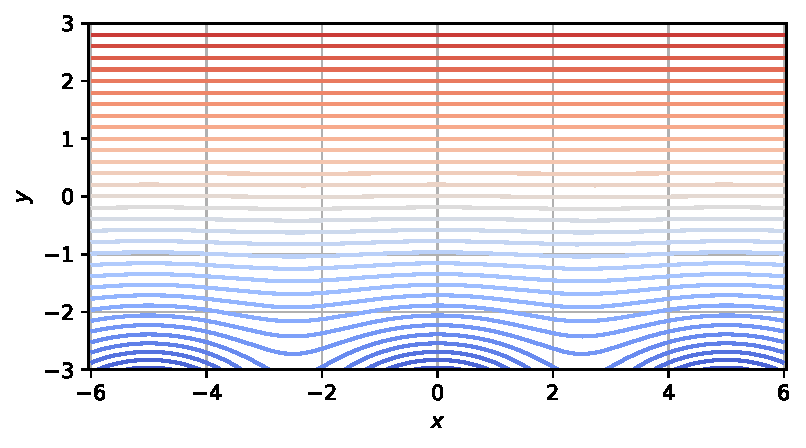
\includegraphics[width=\textwidth]{papers/ueberschall/figures/Stromlinien.pdf}
    \caption{Stromlinien über dem Wellblech für $\frac{A}{U}=0.2$.}
    ~\label{fig:stromlinien}  
\end{figure}

Mit Hilfe der Bernouilli'schen Gleichung
\begin{align*}
    p_{tot}
    =
    \frac{1}{2}\,\rho\,V^2
    +
    p
    +
    \rho\,g\,z,
\end{align*}
wobei $p_{tot}$ der Totaldruck ist, welcher
auf einer Stromlinie konstant ist.
$\rho$ die Dichte des Fluids, $g$ die Erdbeschleunigung,
$V$ die Geschwindigkeit an einem Ort auf der Stromlinie
und $z$ gemäss (cite Wikipedia).
Der letzte Term fällt wegen $z=0$ weg, da wir nur in 
der $x,y$-Ebene arbeiten.
Übrig bleibt dann noch
\begin{align*}
    \underbrace{p}_{\text{statischer Druck}} 
    +
    \underbrace{\frac{1}{2}\,\rho\,v^2}_{\text{dynamischer Druck}}
    =
    \mathrm{const},
\end{align*}
was nichts anderes sagt als, dass der statische Druck und der 
dynamische Druck zusammen überall gleich sind auf einer Stromlinie.
Wenn wir nun den lokalen Druck $p(x,y)$ in unserem Fall berechnen wollen,
dann nehmen wir die Strömungsgeschwindigkeit $U$ als Referenz.
Das sieht dann folgendermassen aus:
\begin{align*}
    p_\infty
    +
    \frac{1}{2}\,\rho\,U^2
    =
    p(x,y)
    +
    \frac{1}{2}\,\rho\,V^2(x,y),
\end{align*}
umgestellt nach dem lokalen Druck
\begin{align*}
    p(x,y)
    =
    p_\infty
    +
    \frac{1}{2}\,\rho\,(U^2-V^2(x,y)),
\end{align*}
wobei $V^2$ nichts anderes ist als
\begin{align*}
    |V(x,y)|^2 = u^2(x,y) + v^2(x,y).
\end{align*}
Damit kann nun die Druckverteilung über dem Wellblech visualisiern,
wie in Abbildung~\ref{fig:druckverteilung}.
Es handelt sich hierbei um den relativen Druck,
d.h es ist abhängig vom Umgebungsdruck.
Man sieht deutlich, dass der höchste Druck an den konkaven Stellen herrscht,
während bei den konvexen Stellen der niedrigste ist.
\begin{figure}
    \centering
    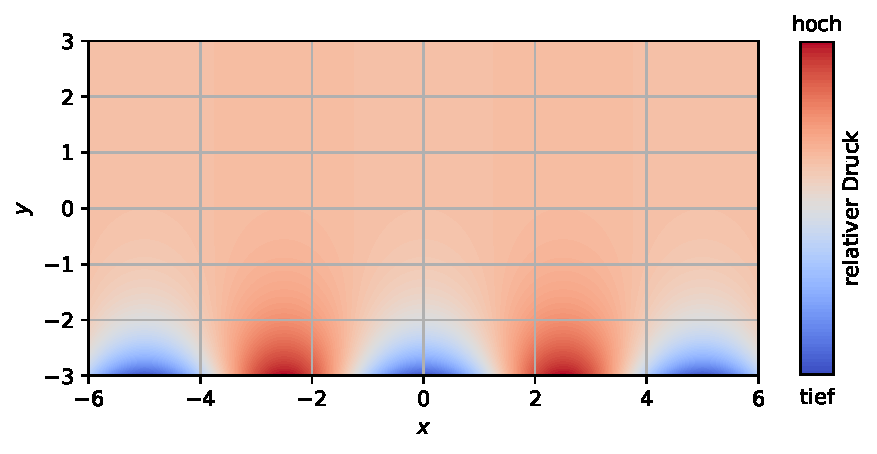
\includegraphics[width=\textwidth]{papers/ueberschall/figures/Druckverteilung.pdf}
    \caption{Relative Druckverteilung über dem Wellblech.}
    ~\label{fig:druckverteilung}  
\end{figure}

\subsection{Kompressible Strömung}
Bei der kompressible Strömung ist das Ganze ein bisschen schwieriger.
Die Ausgangslage ist eine komplexere partielle 
Differentialgleichung zweiter Ordnung, welche vereinfacht
wurde indem sie lediglich auf die Ausdrücke reduziert, die 
die grösste Abweichung bedingen.
Das Vorgehen dafür ist in~\cite{Ackeret1928} ausführlich dokumentiert.
Es handelt sich daher nur um eine Näherungslösung,
die aber einige wesentlichen Züge der wahren Lösung wiederspiegelt.
Die Näherungsgleichung lautet:
\begin{align*}
    \frac{\partial\,^2\,\Phi}{\partial\,x\,^2}\,
    \left(1-\frac{U^2}{a^2}\right)
    +
    \frac{\partial\,^2\,\Phi}{\partial\,y\,^2}
    =
    0
\end{align*}
Der Ausdruck in der Klammer ist eine Konstante, d.h.
durch eine einfache Koordinatentransformation
\begin{align*}
    x 
    &=
    \xi \\
    y\,\beta
    &=
    \eta,
\end{align*}
wobei
\begin{align*}
    \beta
    &=
    \sqrt{1-\frac{U^2}{a^2}}
\end{align*}
ist.
Das führt dann wenig überraschend zu
\begin{align*}
    \frac{\partial\,^2\,\Phi}{\partial\,\xi\,^2}\,
    +
    \frac{\partial\,^2\,\Phi}{\partial\,\eta\,^2}
    =
    0,
\end{align*}
der gewöhnlichen Laplace'schen Gleichung, wie
bei der Potentialströmung.
Das Potential dieser kompressiblen Strömung ergibt sich zu
\begin{align*}
    \Phi
    =
    U\,x + A\,\frac{l}{2\,\pi}\,\sin\left(\frac{2\,\pi\,x}{l}\right)
    \,e^{-\frac{2\,\pi\,y\,\beta}{l}}
\end{align*}
\begin{align*}
    \Phi
    =
    U\,x + U\,\frac{h}{\beta}\,\sin\left(\frac{2\,\pi\,x}{l}\right)
    \,e^{-\frac{2\,\pi\,y\,\beta}{l}}
\end{align*}
und die dazugehörige Stromfunktion
\begin{align*}
    \Psi(x, y)
    =
    U\,y - U\,\frac{h}{\beta^2}\,\cos\left(\frac{2\pi x}{l}\right)
    \,e^{-\frac{2\pi y \beta}{l}}.
\end{align*}
